\chapter{Conclusion}

\section{Summary}
The project aimed to construct a language for Turing Machines that abstracts Turing Machine operations, and investigate whether it is easier to learn the concept by pen-and-paper or through programming. To achieve this, the project as split into 3 phases:
\begin{itemize}
    \item defining the language;
    \item constructing a parser for the language;
    \item showcasing the parser in a website (the product).
\end{itemize}
The 3 phases were completed, after which there was an evaluation session aimed at comparing the teaching of Turing Machines using diagrams and programs.

The user evaluation showed that students find the language somewhat easier to understand and than Turing Machines. However, due to the limited nature of the evaluation and the previous programming experience of the students, this result might not hold in general.

\section{Future Work}

There are many additions that can be made to the language and the product in future. These will help further abstract the TM operations.

\subsection{Language}
Although the language is equivalent to TMs and has abstracted many aspects of TM states and transitions, it is still quite low-level and could abstract the operations further. There are many common paradigms that can be added to the language. These include:
\begin{enumerate}
    \item the ability to traverse to the end (or the start) of the tape string in one command, e.g. \texttt{move end}; 
    \item an \textit{else} block (an \textit{if} block for the remaining letters); and
    \item the ability for modules to be parameterised with respect to letters.
\end{enumerate}
We illustrate these issues with the following program:
\lstinputlisting[language=TML]{code/fut_work_tml.txt}

The first feature is a very common feature found in programs- many programs involving some check on the final character. For example, in the program above, we are traversing to the end twice- at lines 5-9 and 17-21. Hence, this would be a highly beneficial feature to add. Instead of abstracting TM operation, this command would actually abstract \textit{tape} operation \emph{move}. However, this command would make programs much more readable, is quite command, and does not abstract the operation much!

The second point is also somewhat common and was suggested by a student. At many points during execution, we want to do something for a single letter and something different for the other letters. For instance, in the example above, at lines 10-13, we want the program to accept the string if and only if the letter is a \texttt{b}. If the alphabet was longer, this would be quite inefficient. Also, another point that was raised during the evaluation sessions was that the language only makes use of pattern-matching, and could further abstract the TM transition function. So, this would be a great feature to extend the language. 

The final feature is quite interesting. There are many programs where the modules are very similar and only differ in some letters. For example, the program above has 2 essentially mirrored blocks at lines 4-16 and 16-28. In fact, the only difference in these lines of code is at lines 10/12 and 22/24, where the letters \texttt{a} and \texttt{b} are the other way round. Hence, adding this feature would make many programs in TML shorter and less repetitive! Moreover, this would further abstract the TM transition function like variables in the WB3 language, while not providing the same flexibility. This means that it is still quite straightfoward to convert from a TML program to a TM.

One of the proposals in the user evaluation was to add the \texttt{shift} command. This command would allow tape values to be shifted by one position to the left or the right. This command is quite useful when we want to introduce a blank entry at the middle of the tape. By adding this command, many complex programs will become easier to reason! However, this feature will \textbf{not} be added since it goes against the purpose of the language. This is because this feature abstracts tape operations \textit{too much}. That is, adding this operation would simplify the TML programs to an unacceptable level. Moreover, there is no such alternative in TMs. As such, it becomes much harder to convert a TML program to a TM!

 \subsection{Product}
There are many possible improvements to the website. These are some of the features that can be added:
\begin{itemize}
    \item support for direct execution of a TM;
    \item a play button on the tape section to execute long programs on long tapes without pressing the step button many times; and
    \item the ability to collapse the panels.
\end{itemize}
All of these are great features that could be added to the website and would make it easier to use!

\begin{figure}[htb]
    \centering
    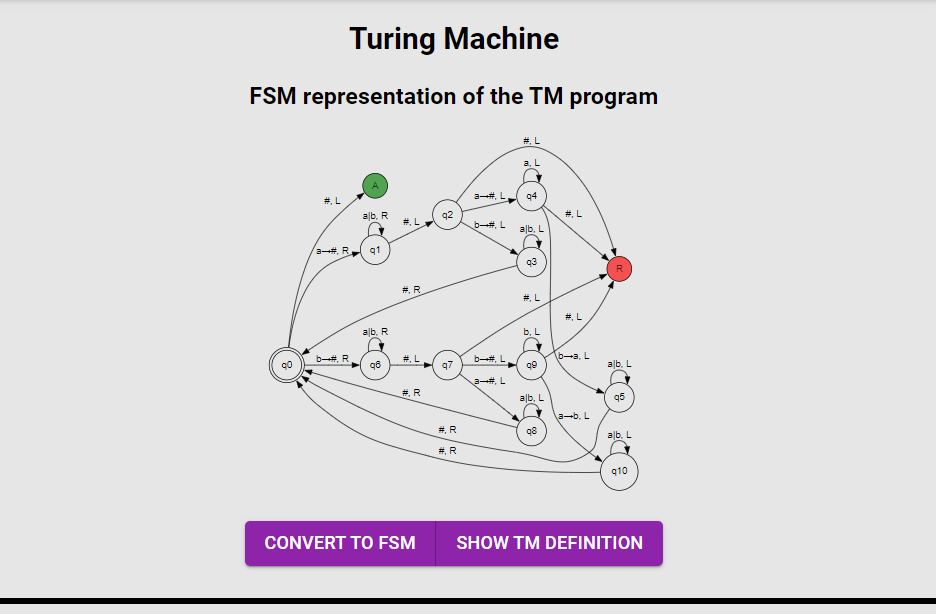
\includegraphics[scale=0.3]{images/Bad FSM visualisation.png}
    \caption{A FSM rendering by graphviz.}
    \label{fig:bad_graphviz_fsm}
\end{figure}

We could also improve the website by making the TM panel more responsive. The FSM is currently being produced using the \textit{graphviz} API. The resulting SVG has hard-coded dimensions, which makes it hard to make the panel responsive. It is not completely possible fix the graph dimensions; only the maximum size of the SVG can be specified. Moreover, the constraints are not taken into consideration when the API produces the FSM. This means that for complex TM, the states are quite small and hard to see- an example is given in \ref{fig:bad_graphviz_fsm}. This makes it hard to follow the execution process. To fix this, we could add one of the following features:
\begin{itemize}
    \item the FSM might produced as it currently is, but the user can zoom in and drag the FSM panel; or
    \item the FSM might be produced so that the states always have the same size, but the user can scroll the panel. 
\end{itemize}
The graphviz framework makes use of the \emph{4-pass algorithm} to render directed graphs \citep{gansner1993technique, gansner2006drawing}, so it is also possible to implement the algorithm directly.

\section{Reflection}
This project was an enjoyable experience for me. I was very happy to work on a self-defined project and that gave me a lot of motivation to work on it! It was also exciting connecting programming languages and Turing machines! This project has also taught me a lot about web development, in particular the React framework.

I do feel that due to the time constraints, I was not able to develop the language and the product completely. There are many extensions that I would have liked to add. Nonetheless, I plan to work on adding these extensions during the summer!
